\documentclass[a4paper, 11pt]{article}
\usepackage{graphicx}
\usepackage{url}
\usepackage{hyperref}
\usepackage[numbers]{natbib}
\usepackage{tabularx}
\usepackage{amsmath}
\usepackage{amssymb}
\usepackage{epstopdf}
\usepackage{inputenc}
\usepackage{geometry}
\usepackage{alphabeta}
\usepackage{float}
\usepackage{changepage}
\usepackage{lipsum}
\usepackage{subcaption}

\setlength{\oddsidemargin}{0mm}
\setlength{\evensidemargin}{-14mm}
\setlength{\marginparwidth}{0cm}
\setlength{\marginparsep}{0cm}
\setlength{\topmargin}{2mm}
\setlength{\headheight}{0mm}
\setlength{\headsep}{0cm}
\setlength{\textheight}{240mm}
\setlength{\textwidth}{168mm}
\setlength{\topskip}{0mm}
\setlength{\footskip}{10mm} 

\newcommand{\code}[1]{\texttt{#1}}
\newcommand{\refsec}[1]{\mbox{Section~\ref{sec:#1}}}
\newcommand{\refapp}[1]{\mbox{Appendix~\ref{sec:#1}}}
\newcommand{\refeqn}[1]{\mbox{(\ref{eqn:#1})}}
\newcommand{\reffig}[1]{\mbox{Figure~\ref{fig:#1}}}
\newcommand{\ud}{\mathrm{d}}                    % upright d (derivative)

\newcounter{foo}
\newcounter{bar}

\title{
    ENEL420 - Genetic Algorithms in Digital Signal Processing\\
    \vspace{1cm}
    \begin{large} 
        Department of Electrical and Computer Engineering\\
        University of Canterbury\\
    \end{large}
    \vspace{1cm}
}

\author{
    \small {Luke Trenberth (ID: 47277086)}\\
    \small {Hassan Alhujhoj (ID: 35352633)}\\
    }
\vspace{2cm}

\date{\small\today}
\begin{document}
\maketitle

\vspace{4cm}
\begin{abstract}
    Genetic Algorithms (GA's) are an evolutionary algorithm, evolving a population of solutions for an optimised 
    solution. This relies on Darwins's Theory of Natural Selection, where he claimed that natural variation, which exists in
    all populations, improve the gene pool amongst, forming the basis for evolution. Genetic Algorithms mathematically 
    formulates this theory, which allows its application to areas in Digital Signal Processing such as 
    Finite Impulse Response Filters, investigated throughout this report. A genetic algorithm was designed to remove
    interference signals from an electrocardiogram (ECG) data signal without data training. 
    
\end{abstract}

\pagebreak
\pagenumbering{roman}
\tableofcontents
\pagenumbering{arabic}
\pagebreak

\section{Introduction}\label{sec:intro}
    Genetic Algorithms (GA) are inspired by the mechanism of natural selection where the strongest and fittest
    individuals would likely be the winners in a competing environment. Genetic Algorithm is used as a direct 
    analogy of such natural evolution where it presumes that a potential solution of a problem is an individual 
    and can be represented by a set of parameters. These sets of parameters are regarded as the genes of a chromosome 
    and can be structured by a string of values in binary form. A fitness value is used to reflect the degree of 
    goodness of the chromosome for the problem which would be highly related with its objective value \cite{Man1997}.
    \\\\
    History has shown that the fitter chromosome tends to yield good quality offspring which means a
    better solution to the problem. Practically, a population pool of chromosomes must be randomly set initially. 
    The size of this population varies from one problem to the other. Each cycle of genetic operation is termed as 
    an evolving process where a subsequent generation is created from the chromosomes in the current population.  
    This evolving process can only be succeeded if a group of those chromosomes, which are generally called
    “parents” or a collection term “mating pool” are selected. The genes of the parents are then mixed to produce 
    offspring in the next generation. From this manipulation of genes process, the “better” chromosome will create a 
    larger number of offspring, and thus has a higher chance of survival in the subsequent generation, emulating the 
    survival-of-the-fittest mechanism in nature \cite{Man1997}.
    \\\\
    To make sure the desired termination criterion is reached, the cycle of evolution is repeated. The offspring of 
    the previous generation are reinserted into the model, further yielding higher quality offsprings \cite{Man1997}.
    \\\\
    There are two fundamental operators that facilitate the evolution cycle: Crossover and Mutation. Both operators 
    are required for such a process even though the selection routine. To further illustrate the crossover procedure, 
    the one-point crossover mechanism is shown in Figure \ref{Fig:crossover}. Genes are exchanged between parents to form 
    offspring. Mutations are randomly generated after crossover with a small probability of occurrence.
    
    \begin{figure}[h!]
        \centering
        \graphicspath{{./wiki/}}
        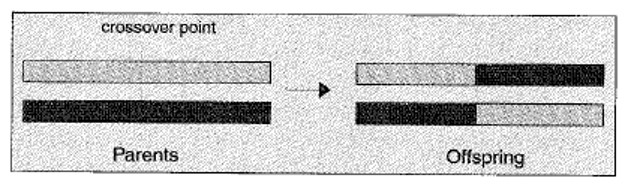
\includegraphics[scale=0.7]{crossover.png}
        \caption{Interference frequencies present in the ECG signal.}
        \label{Fig:crossover}
    \end{figure}

\section{Background}\label{sec:bg}
    \subsection{Digital Signal Processing of ECG Signals}\label{sec:bg_sub1}
        In assignment one, a noisy ECG signal with 1024Hz sampling frequency was provided to be filtered. 
        The assignment required the implementation of a notch filter with either an FIR or IIR filter.
        An FIR or IIR notch filter was suited to filter this ECG signal since there were a clear two 
        interference frequencies present within the frequency spectrum of the ECG signal.
        These interference frequencies were identified to be $f_{1} = 31.456Hz$ and $f_{2} = 74.36Hz$
        as shown in Figure \ref{Fig:rejFreq}. Interference frequencies from other ECG signals can be found to
        be between $30Hz \leqslant f \leqslant 100Hz$. It should be noted that the first peak in Figure \ref{Fig:rejFreq} is the 
        DC component due to the use FFT to get the frequency response of the time domain ECG signal.
        \\
        \begin{figure}[h!]
            \centering
            \graphicspath{{./wiki/}}
            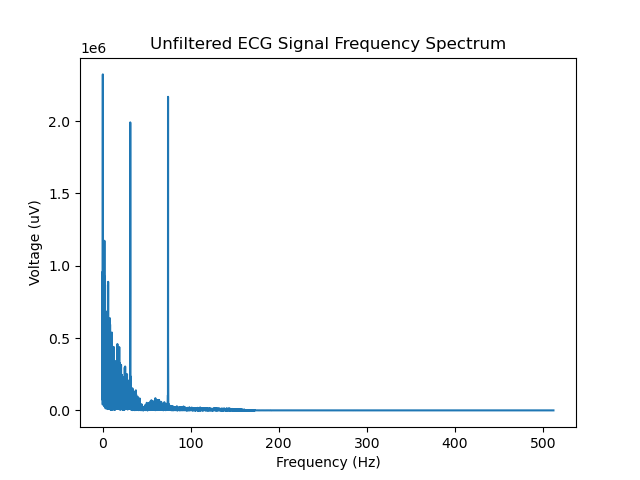
\includegraphics[scale=0.6]{ECG_freq_spectrum.png}
            \caption{Interference frequencies present in the ECG signals.}
            \label{Fig:rejFreq}
        \end{figure}
        \\
        One method to filter these two frequencies was to reject them with either a window or Parks-McClellan filters.

    \subsection{Genetic Algorithms}\label{sec:bg_sub2}
    Since the emergence of Darwin's theory of natural selection, GA has become a powerful tool and used in various
    applications.  The GAs are also known as optimisation algorithms. Optimisation algorithms have two major classes.
    These two classes are classified as calculus-based techniques and enumerative techniques. Calculus-based
    optimisation algorithms employ the gradient-directed searching mechanism to solve error surfaces or differentiable
    surfaces of an objective function. A common misuse of an objective function can occur with an ill-defined or multimodal
    objective function. This can lead to obtaining a local optima instead of a global optima. Such use of objective
    functions are common in signal processing \cite{Tang1996}.
    \\
    \begin{figure}[h!]
        \centering
        \graphicspath{{./wiki/}}
        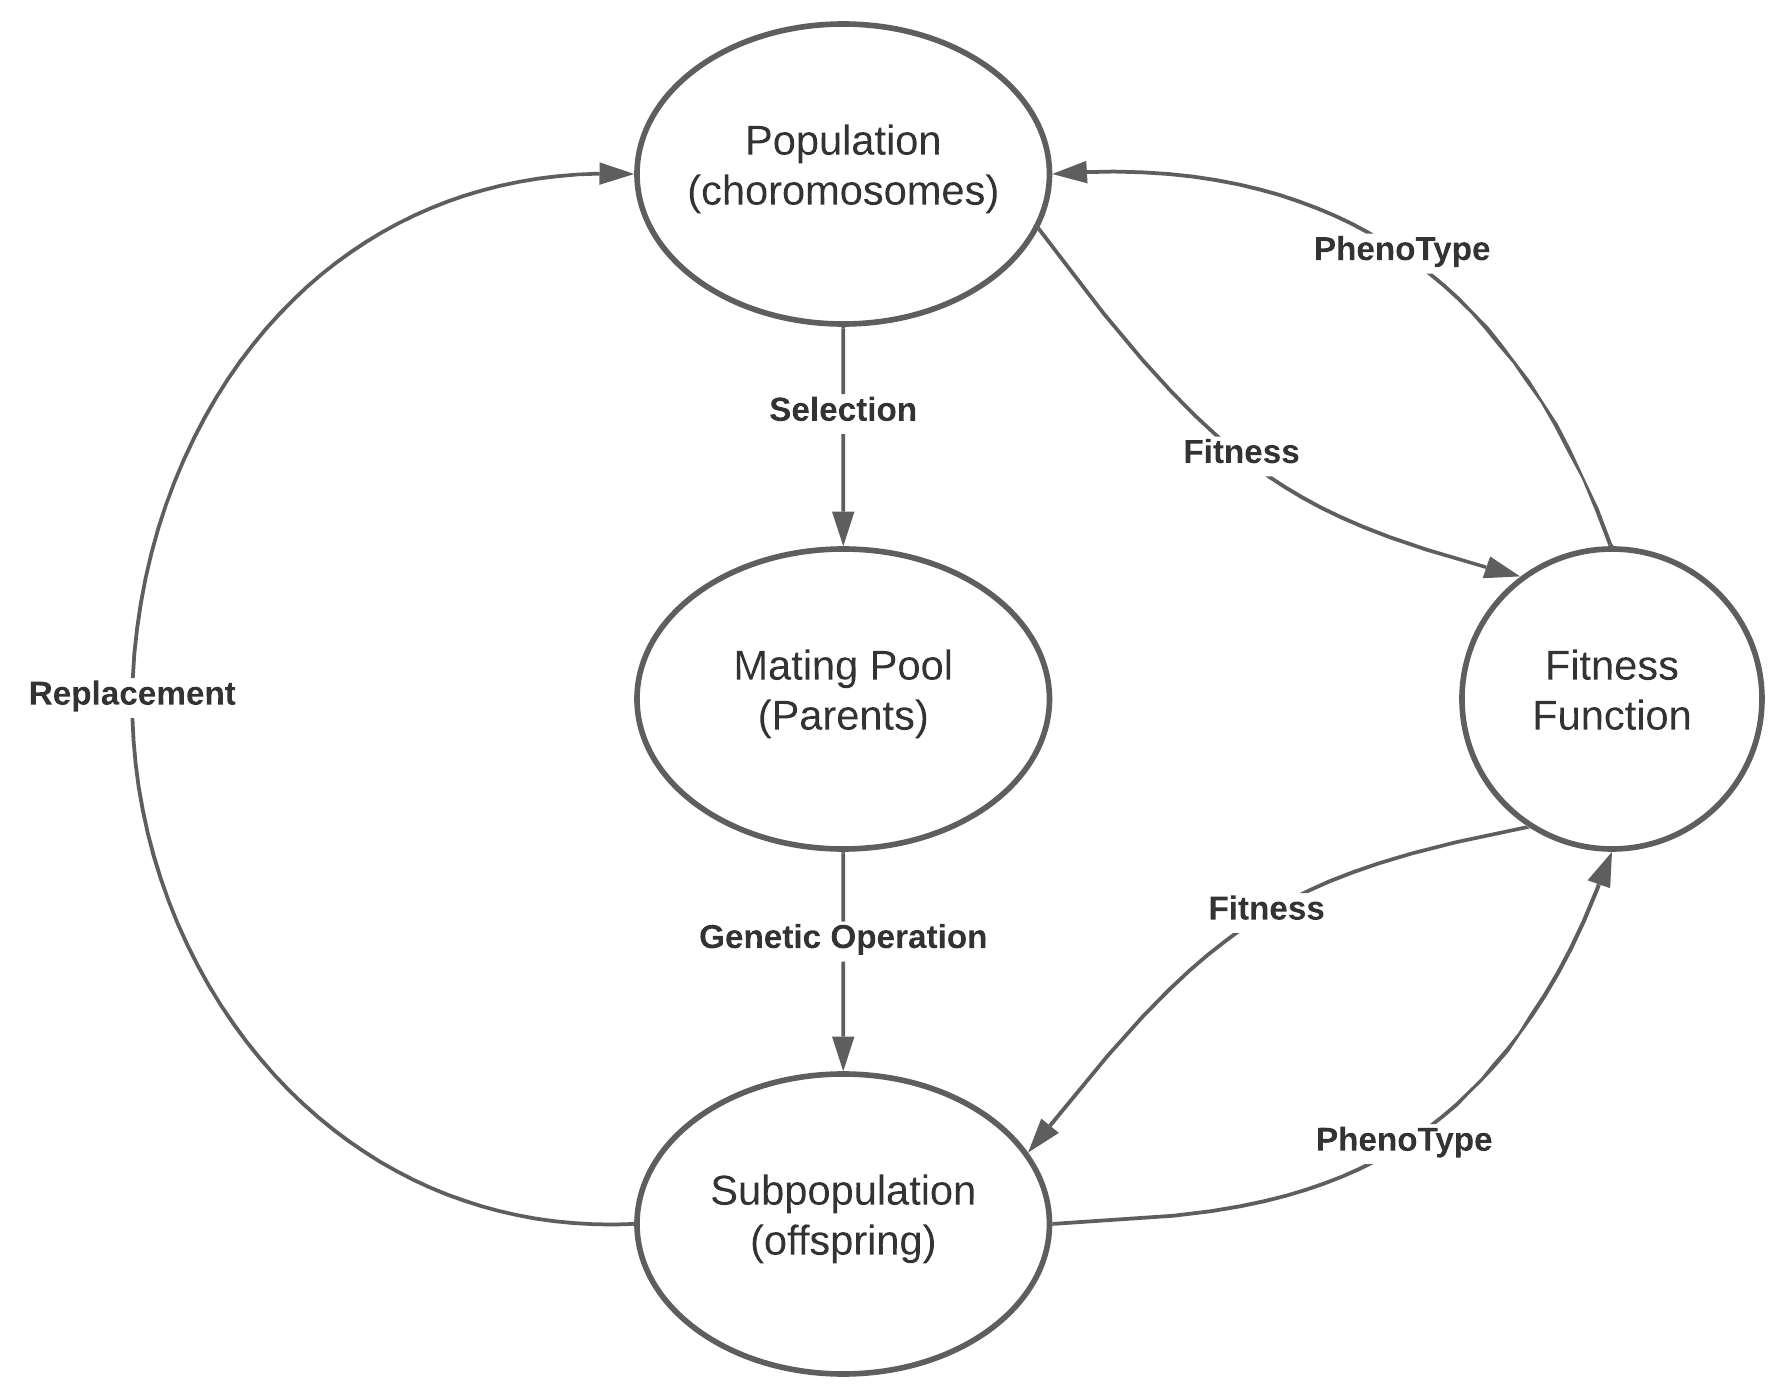
\includegraphics[scale=0.7]{GA_cycle.png}
        \caption{Genetic Algorithms cycle. Adapted from \cite{Tang1996}, refer to Figure 1}
        \label{Fig:GA_cycle}
    \end{figure}
    \\
    Genetic Algorithms have a general cycle known as GA cycle, shown in Figure \ref{Fig:GA_cycle}. This cycle is a searching
    process  based on the laws of natural selection and genetics. A simple GA consists of three operations: Selection, Genetic
    Operation and Replacement. GA population comprises of a group of chromosomes from which candidates can be selected for the
    solution of a problem. The population, initially, is generated randomly. The fitness values of all chromosomes are 
    evaluated by calculating the objective function in a decoded form (phenotype). to generate the offspring by the defined 
    genetic operations, a particular group of chromosomes (parents) are selected from the total population. The fitness of the 
    offspring is evaluated in a similar fashion to their parent chromosomes. The chromosomes in the current population are then 
    replaced by their offspring based on a certain replacement strategy defined by the user \cite{Tang1996}.
    \\\\
    This GA cycle is then repeated until a desired termination criterion is reached. For example a predefined number of generations
    is produced. If all goes well and according to this process of simulated evolution, the best chromosomes is the final population 
    can become a highly evolved solution to the problem. Generally, GA follows the following process \cite{Tang1996}.

    \begin{enumerate}
       \item Randomly generate an initial population $X(O):= (x_{1}, x_{2}, ..., x_{N})$.
       \item Compute the fitness $F(x_{i})$ of each chromosome $x_{i}$ in the  current population $X(t)$;
       \item Create new chromosomes $X_{r}(t)$ by mating current chromosomes, applying mutation and recombination (crossover) as the 
       parent chromosomes mate;
       \item Delete numbers of the population  to make room for the new chromosomes;
       \item Compute the fittness of $X_{r}(t)$, and insert these into the popuation;
       \item $t:= t + 1$, if not (end-test) go to step 3, or else stop an dreturn the best chromosome.
   \end{enumerate}

        \subsubsection{Crossover}
            Crossover is a GA operator which is a recombination operator that combines subparts of two parents 
            chromosomes to produce offsprings that contain some parts of both parents' genetic material. Crossover
            is considered by many GA practitioners to be the determining factor that distinguishes the GA from
            all other optimisation algorithms \cite{Tang1996}.

        \subsubsection{Mutation}
            Mutation is another operator that introduces variations into the chromosomes. This variation can be
            local or global. Mutation can occur some occasionally but can randomly alters the value of a string
            position. A randomly generated bit can replace any bit of the chromosome bitstring mutating the original
            bit sequence of the parents \cite{Tang1996}.

        \subsection{Applications}
        Genetic Algorithms are widely used and can be applied in many applications such as in analog signal processing, 
        digital signal processing, DSP MCU scheduling, FIR filter design, PID tuning and PID control, etc 
        \cite{Chen2017, Fleming1993, Cao2012, Fabijanski2008, Miyata2018, Amphlett1996}.
        \\\\
        In \cite{Chen2017}, GA were used to control a BLDC motor with PI speed controller that is then processed by 
        a Digital Signal Processor (DSP). In a real control system, the processing time in a cycle might be token long
        when the data communication is processed. The implementation of a GA-PI control design improves the performance of
        the PI control of the BLDC motor according to \cite{Chen2017}. In this study, the BLDC motor fitness is evaluated
        based on the transfer function of the motor which is then used to evaluate the chromosomes population 


\section{Method}\label{sec:meth}
    In this assignment, genetic algorithms were used to design a bandstop Finite Impulse Response (FIR) filter for Assignment 1's 
    ECG data. To design a filter, the filtered frequencies, the bandwidth and band transition width  were required 
    characteristics. These were set as the genes for the filter and each chromosome contained these parameters.
    A population was then initialised with $p_{size}$ chromosomes, each containing the genes to create a filter. 
    For each chromosome, the filter created by its characteristics, returning a fitness score, with higher scores 
    representing higher quality filters. The genetic algorithm used the fitness scores of the previous generation
    to generate a new generation, where the highest $n_{parent}$ scores become the parents of the succeeding generation. 
    utilising genetic crossover, variation and mutation. An identical process is then conducted on the succeeding generation (Figure \ref{Fig:method_1}). 
    As the number of iterations increases, the population fitness increases. Once $N_{generations}$ have been reached, the
    optimal filter coefficients are returned. 

    \begin{figure}[h!]
        \centering
        \graphicspath{{./wiki/}}
        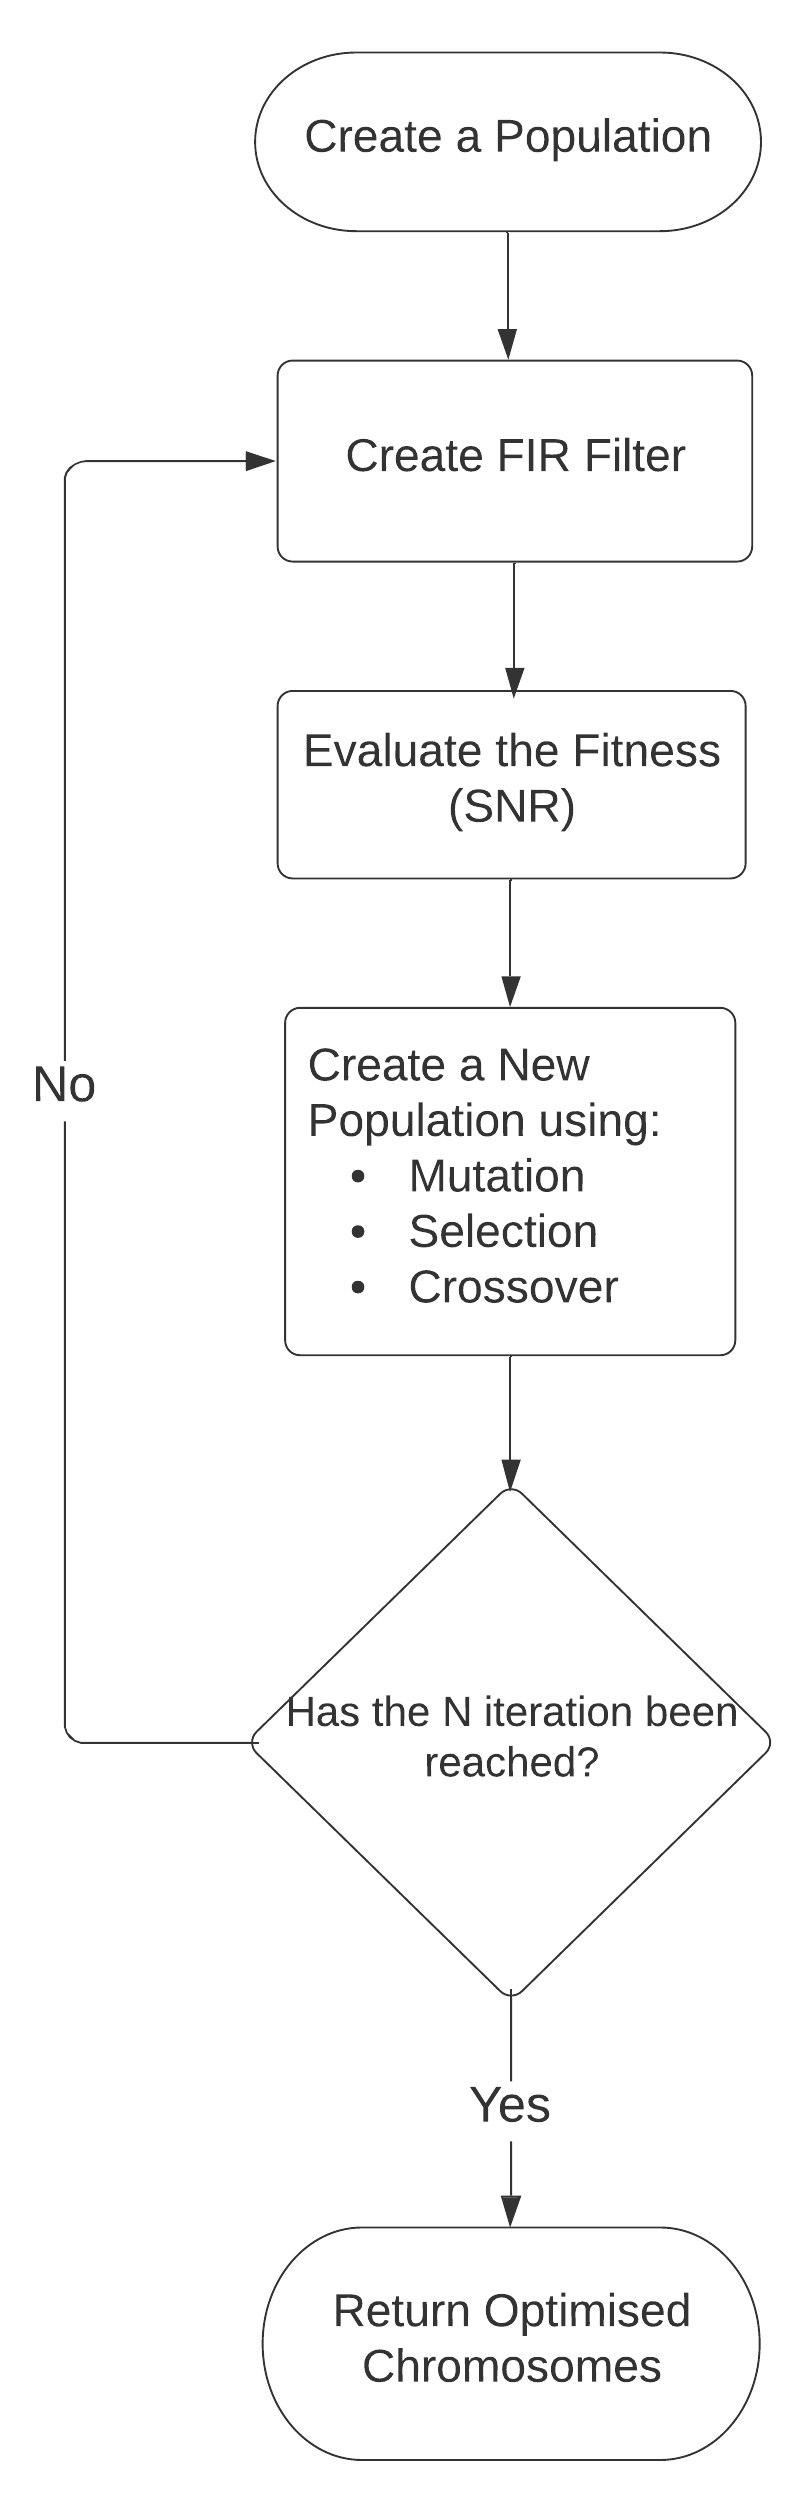
\includegraphics[scale=0.8]{Flowchart.png}
        \caption{Flowchart diagram of the use of GA to process ECG signals.}
        \label{Fig:method_1}
    \end{figure}

    \subsection{Digital Signal Processing Data}\label{sec:meth_sub1}
        Due to accessible data samples, the ECG signals from Assignment 1 have been analysed. This data contained
        two interference frequencies between  $f = 30 - 100Hz$. The interference frequencies must be identified and 
        removed from the data. \cite[]{Garip2018} Each chromosome had a set of genes representing a filter property. The genes were 
        represented as decimal numbers, known as decimal encoding, which is useful in scenarios that require a high
        level of accuracy. 
        \\\\
        A python class was created to analyse the signal. This class was able to convert the time domain signal to the
        frequency domain, giving a plot of the signal. This class was able to conduct filtering techniques such as Window
        Filtering, Frequency Sampling and Parks-McLellan Filtering. Plots of filtered and unfiltered data was generated. 
        This allowed the data to be analysed with a level of abstraction.

    \subsection{Fitness Function}\label{sec:meth_sub2}
        As each characteristic will produce a different gain, it was important to quantify how effective each filter was. 
        The Signal to Noise Ratio (SNR) is considered a useful metric for choosing the most optimal filtering coefficients. 
        For each chromosome, a Parks-McLellan filter was generated, and then applied to the original data. The filtered signal
        power was then calculated by considering the variance in the signal. The difference between the filtered power
        and the original signal power was then considered the noise power, and the signal to noise power was calculated. 
        Signals with higher SNRs were considered more optimal filtering, and therefore the SNR of the signal was determined
        to be an appropriate measure of the sample's fitness. 

        \begin{equation} SNR = var(y_{0}) - var(y)\end{equation}

    \subsection{Population Selection}\label{sec:meth_sub3}
        Parent chromosomes were chosen by taking the chromosomes with the largest fitness scores in the previous generation,
        known as elitest selection. 
        Chromosomes with the largest fitness scores have the most successful genes and were incorporated into the
        successor generation gene pool. For the analysed ECG data set, a population of 20 chromosomes was used, with four
        parents succeeding to the following generation. The effect of modifying each of these results on the success of the
        algorithm and the number of iterations for success was investigated. 
        \\\\
        Successive chromosomes were created through a combination of genetic mutation, and crossover of the parent chromosomes.
        Genetic mutation was incorporated into the genetic algorithm by random variation in the genetic sequences, using numpy's 
        $np.randint()$ function. This allowed the frequency genes to span the entire frequency range. Genetic crossover was implemented
        to find optimal combinations of known genes in the gene pool. This mixes genes from parent chromosomes. The effectiveness of 
        found gene combinations was assessed in the next generation, ideally finding combinations of chromosomes that yield higher 
        fitness. Any combinations with higher fitness than the original are then given a higher selection priority. 

    \subsection{Finite Impulse Response (FIR) Filtering Techniques}\label{sec:meth_sub4}
        While a few filtering techniques have been written into the code, the Parks-McClellan Filter was originally utilized. 
        This algorithm finds the optimal Chebyshev FIR filter using an iterative process. For each interference frequency identified, 
        a Chebychev filter was created. All filters were then convolved to the original data frequency responses. Ideally, this 
        removed the interference at the given frequencies from the signal without affecting the remaining frequency response of the signal.

\section{Results}\label{sec:res}
    When the Genetic Algorithm was run using a Parks-McLellan filter, the algorithm identified the optimal genes for maximum SNR. 
    With the filter population size of $p_{size} = 20$, and a maximum number of generations of $n = 200$, a filtered 
    output was produced. As seen in Figure \ref{Fig:result_1}, the interference frequencies found in the original signal have 
    been removed from the frequency plot. When data from other files was tested, these were also successful without changing 
    parameters. This proved the fitness function was robust as interference frequencies were identified in various conditions
    without needing data training. 
    \\\\
    In the time domain, (Figure \ref{Fig:result_2}) the interference frequencies introduced noise, obstructing the true waveform. 
    When the frequencies are removed, the signal is much clearer, resulting in more useful information due to the filtering. 
    
    \begin{figure}[h!]
        \centering  
        \begin{subfigure}[b]{0.5\linewidth}
            \graphicspath{{./wiki/}}
            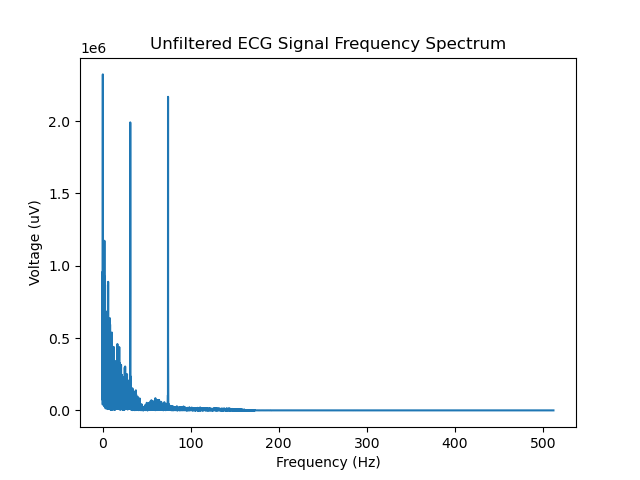
\includegraphics[width=\linewidth]{ECG_freq_spectrum.png}
        \end{subfigure}%
        \begin{subfigure}[b]{0.5\linewidth}
            \graphicspath{{./wiki/}}
            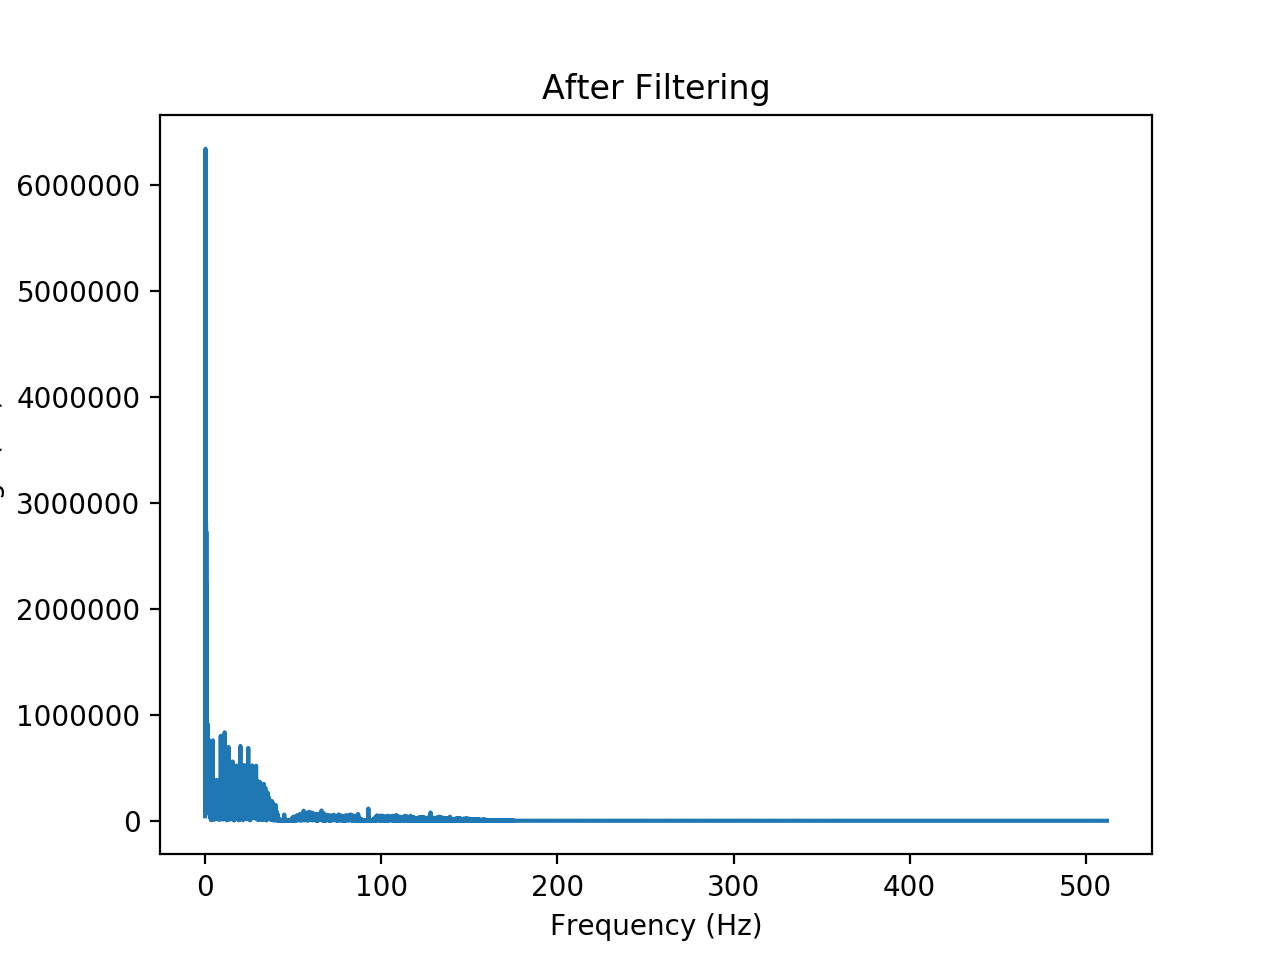
\includegraphics[width=\linewidth]{af_filtering_1kGen20Pop.png}
        \end{subfigure}
        \caption{The filtered output of ECG signal 1, using $p_{size} = 20$, $n = 1000$.}
        \label{Fig:result_1}
    \end{figure}

    \begin{figure}[h!]
        \centering  
        \begin{subfigure}[b]{0.5\linewidth}
            \graphicspath{{./wiki/}}
            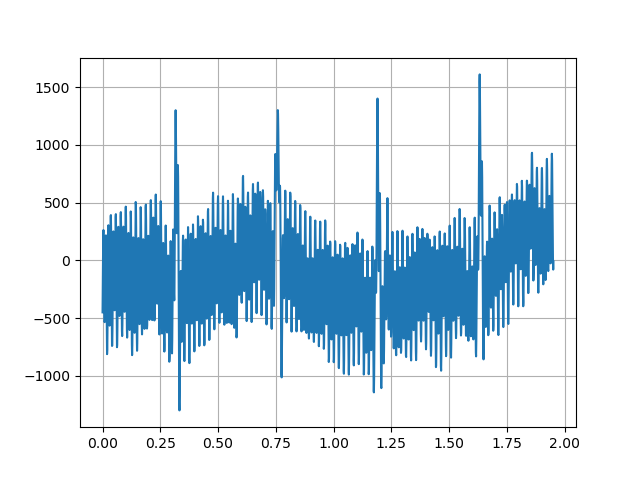
\includegraphics[width=\linewidth]{TDU.png}
        \end{subfigure}%
        \begin{subfigure}[b]{0.5\linewidth}
            \graphicspath{{./wiki/}}
            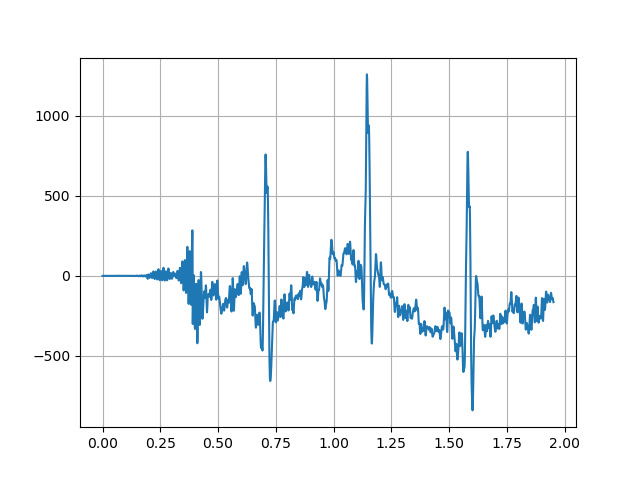
\includegraphics[width=\linewidth]{TDF.png}
        \end{subfigure}
        \caption{The unfiltered (left) and filtered (right) time domain signal, 
        seen above with parameters $p_{size} = 20$, $n = 1000$.}
        \label{Fig:result_2}
    \end{figure}

    When varying the number of generations with the population size, the maximum fitness was consistently reached within 5 
    iterations (Figure \ref{Fig:result_2}). However, when the population size was decreased, a larger number of
    iterations was required to reach optimum fitness. Using $p_{size} = 20$, $n = 50$ gave reasonable filter results with a
    small execution time \cite[]{Garip2018}.

    \begin{figure}[h!]
        \centering
        \graphicspath{{./wiki/}}
        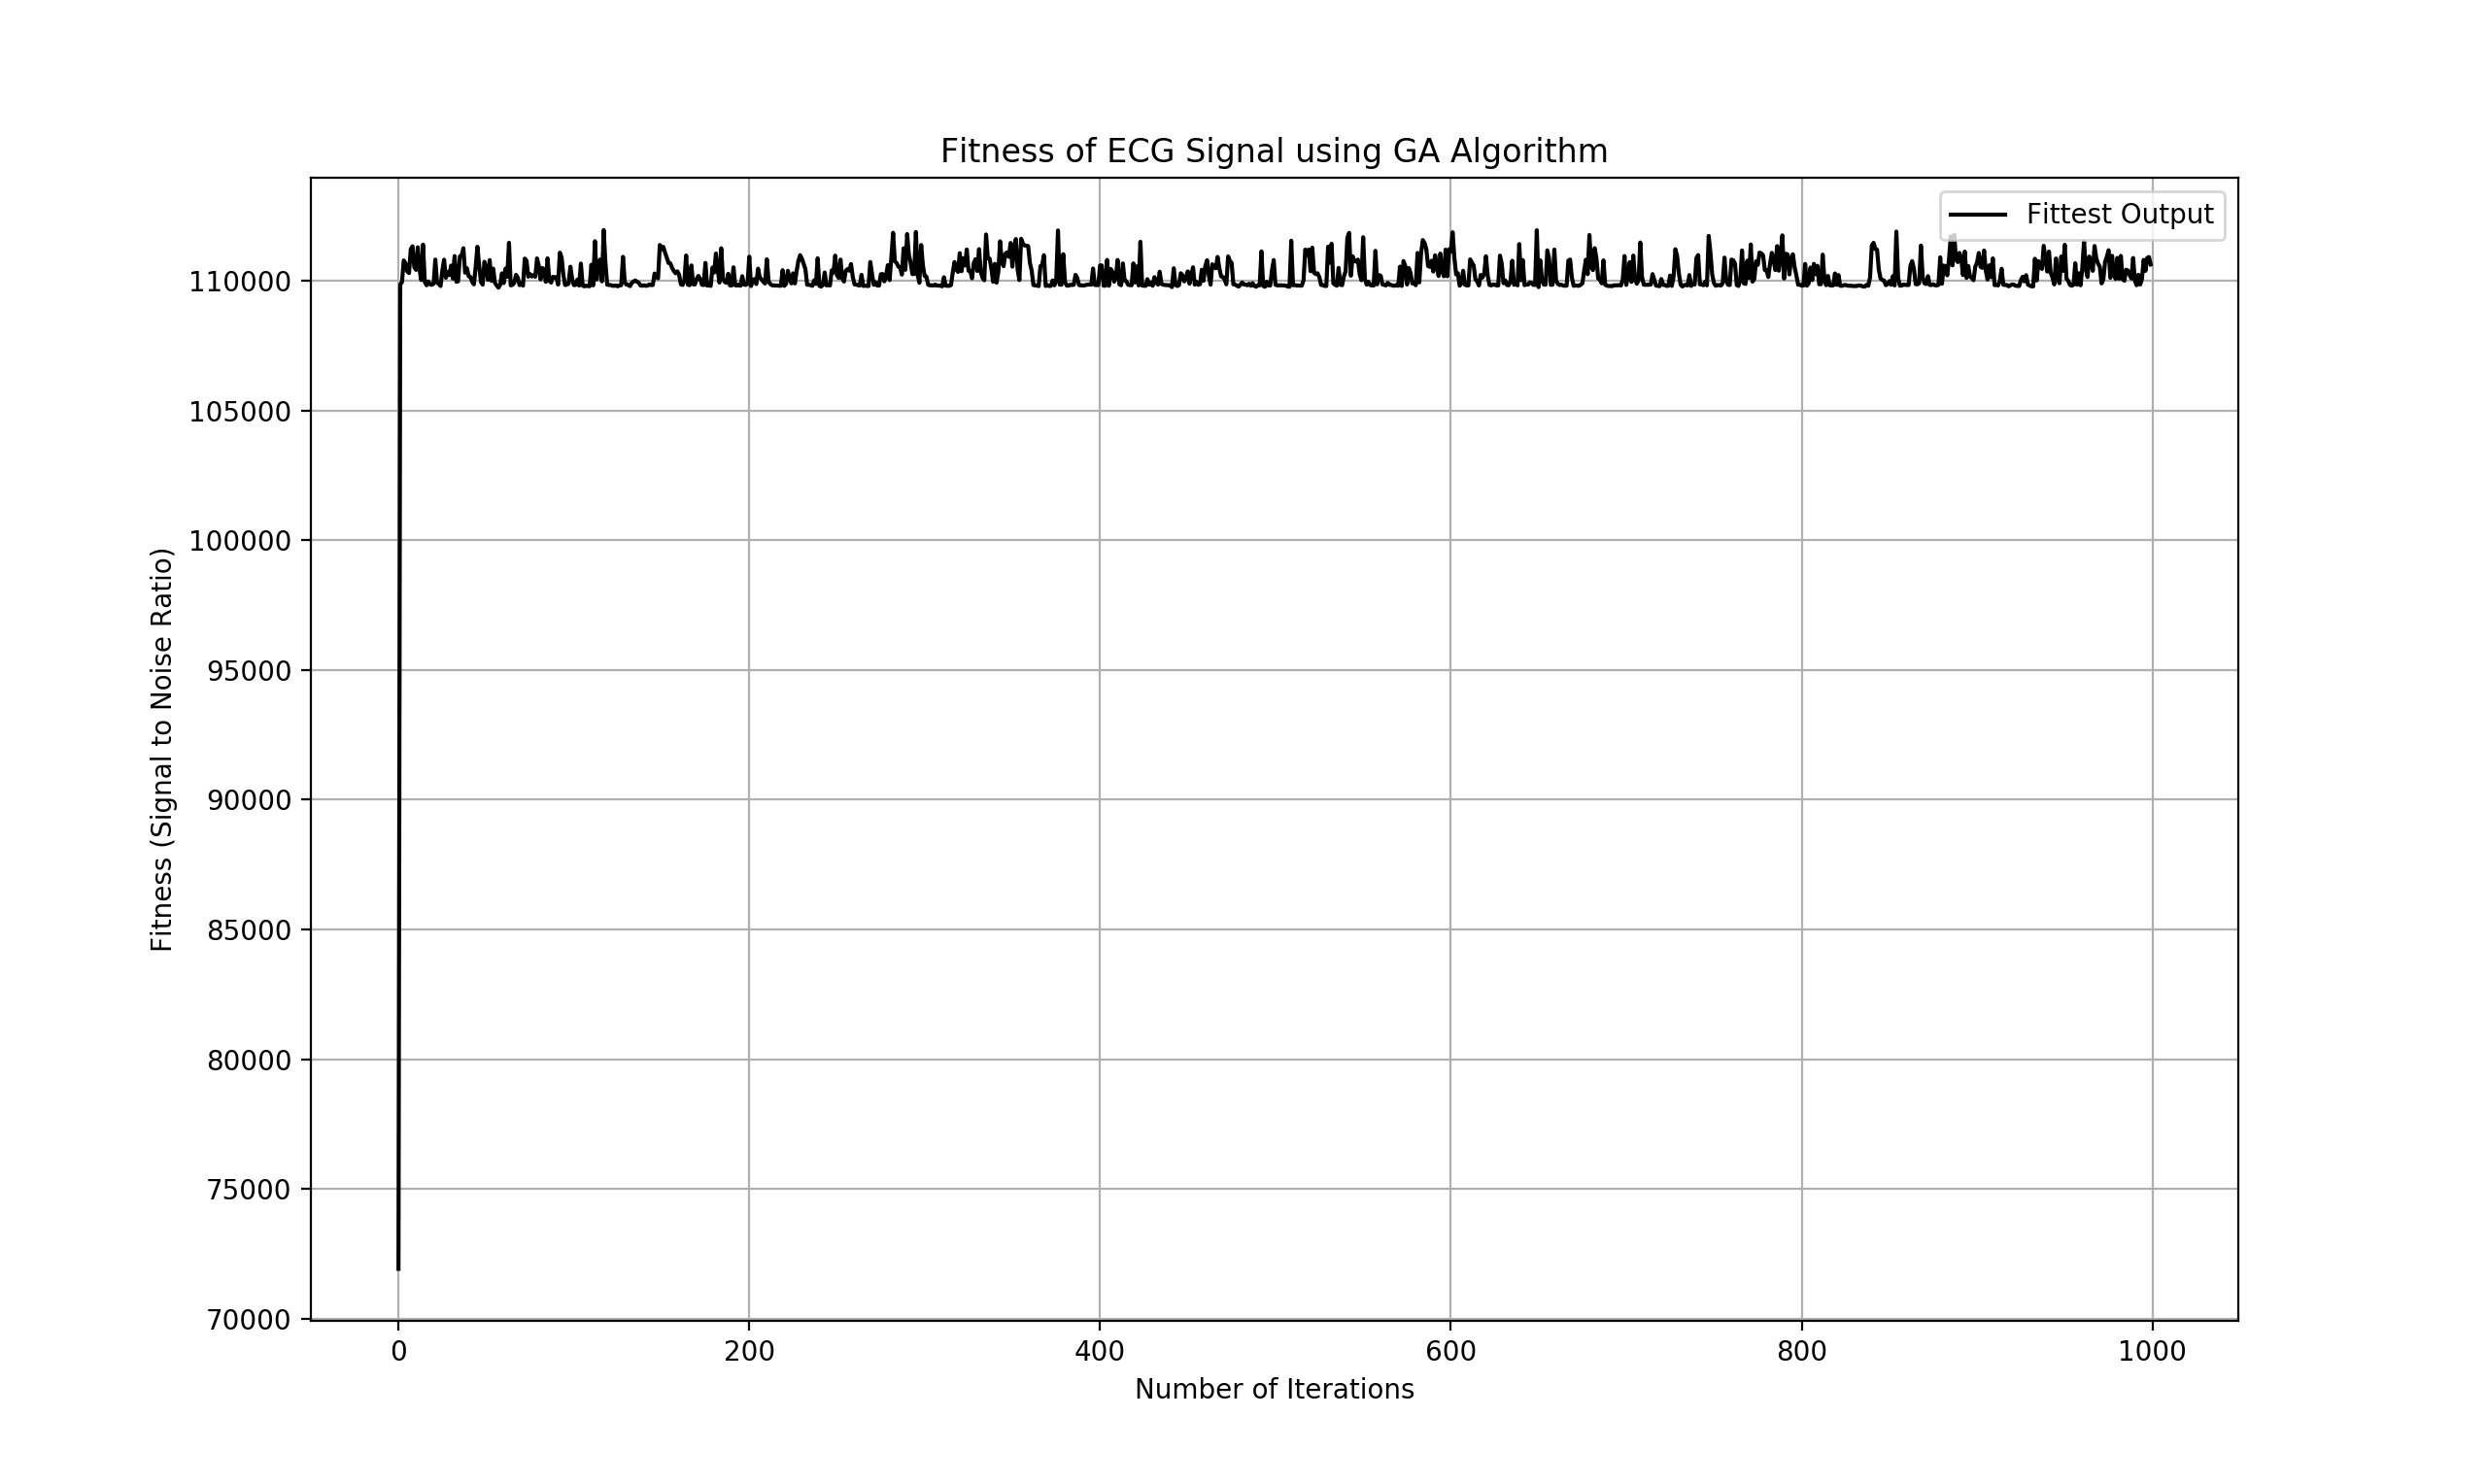
\includegraphics[scale=0.5]{1kGen20Pop.png}
        \caption{The population fitness of ECG signal 1 through iterations, using $p_{size} = 20$, $n = 1000$.}
        \label{Fig:result_2}
    \end{figure}

\section{Discussion}\label{sec:dis}
    The Genetic Algorithm has been effective at identifying and filtering the interference frequencies. These algorithms 
    allow quick identification of required parameters without a comprehensive understanding of the system. Genetic Algorithms 
    provide flexible, robust solutions to filter design. These can also be applied to with varying parameters without requiring
    mathematical derivations. Unlike other iterative methods, Genetic Algorithms can span the entire solution space to find
    optimal solutions, and when given appropriate parameters, the system will not misidentify suboptimal solutions in local
    maximums. However, Genetic Algorithms require a fitness function to assess the quality of each potential solution quickly. 
    This can be difficult in systems that require significant time for data gathering. GA's are also computationally intensive.
    \\\\
    The GA used to design filter coefficients emulates these properties. Once a population and fitness function was created,
    and appropriate system parameters were identified, the algorithm was consistently able to return high-quality filters, 
    removing the interference from the original ECG signal. By inspection, these solutions identified the optimal results to
    high degrees of accuracy. However, the algorithm took a reasonable time to produce results.

    \begin{figure}[h!]
        \centering  
        \begin{subfigure}[b]{0.4\linewidth}
            \graphicspath{{./wiki/}}
            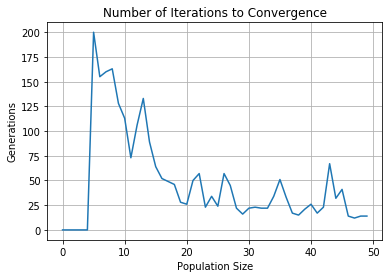
\includegraphics[width=\linewidth]{GenPerPopSize.png}
        \end{subfigure}
        \begin{subfigure}[b]{0.4\linewidth}
            \graphicspath{{./wiki/}}
            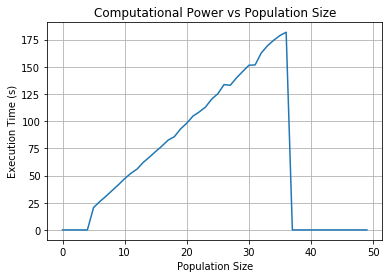
\includegraphics[width=\linewidth]{ExPerPopSize.png}
        \end{subfigure}
        \caption{The effect on the number of required generations (Left) for convergence and execution time (Right) from varying
        population size. }
        \label{Fig:discuss_2}
    \end{figure}

    The effect of varying the parameters used for  the genetic algorithm, such as the number of generations, the population
    size, the number of parents \cite{Garip2018}. It was determined smaller population samples took more iterations to converge
    to a solution, sometimes not converging at the solution. However, large population samples considerably increased execution 
    times. However, the larger the population size used, the more likely the algorithm was to succeed. 
    \\\\
    While using genetic algorithms to complete this problem is possible, this may not always be practical\cite[]{Yu2003}. By 
    visually inspecting the plot in the frequency domain, it is possible to identify the frequencies (albeit to less accuracy), 
    and manually designing a filter to complete this problem. As genetic algorithms do not follow a standard iteration process, 
    often designers can be reluctant to use genetic algorithms. Other iteration techniques could also be used to solve for the 
    maximum such as global convergence. This would be less computationally intensive, however could require more analysis. 
    \\\\
    To improve the filtering capabilities, the filtering method could be incorporated into the chromosomes, which
    would allow the program to identify the optimal filter technique. This would automate the type of filter, allowing
    the program to optimise for the type of filter as well as the filter characteristics. 
\section{Conclusion}\label{sec:conc}
    The purpose of this report was to investigate the applications of genetic algorithms in signal processing. This is an 
    evolutionary algorithm, which uses a population of chromosomes containing a set of genes. The population is evolved
    over a number of generations to optimise for the optimal genes. The fitness function is used to assess the success of each
    chromosome. These are often utilized to optimize analog control signals, PI controllers or FIR filters.  
    \\\\
    Genetic Algorithms were applied to a ECG data signal to filter interference. The genes, consisting of the filtering frequencies, 
    have been used to create a filter. The filter quality has then been assessed by the fitness function, the Signal to Noise
    ratio. The algorithm then completed a set number of evolutions unless a set threshold was reached. 
    \\\\
    The genetic algorithm parameters have also been analysed. It was found the larger the population size the less generations
    required for convergence to the optimal solution. Furthermore, the larger the number of generations completed, the larger
    the execution time of the algorithm. 
    \\\\
    Genetic Algorithms do not require complex understandings of the dynamics of a system, and are able to span the entire
    genetic range, which prevents genetic algorithms finding suboptimal solutions given appropriate input parameters. However, 
    genetic algorithms are computationally expensive, which can limit their applications.  

    

\pagebreak
\bibliographystyle{IEEEtran}
\renewcommand{\bibname}{References}
\renewcommand{\bibsection}{\section{\bibname}}
\renewcommand{\cite}{\citep}
\bibliography{ref}
\pagebreak

\end{document}

